\section{Network Service Orchestration}
\label{sec:nso}

\subsection{Definitions}%%%%%% Change the title %%%%%%
%\subsection{Orchestration: Definitions} 
\label{sec:orchdef}

Various communities differ concerning the meaning, assumptions, and scope of orchestration functions. Thus, it is helpful to begin by reviewing the community understanding to get the main concepts and significance. To this end, we overview the leading organizations and efforts defining the term Orchestration in the context of network service.



%text libreoffice 
\gls{nist} \cite{Bohn2011NISTArchitecture} was one of the first organizations to define the concept of Service Orchestration formally. According to NIST vision, orchestration is a process related to the arrangement, coordination, and management of virtualized infrastructure to provide different cloud services to customers.

A couple of years ago, the term orchestration was adopted by \gls{etsi} in the scope of \gls{nfv}. In \gls{etsi} \gls{nfv}, the meaning of orchestration leads to a vague distinction between orchestration and management. According to~\cite{ETSIISG2018}, the orchestration is a set of coordinated processes that automate the management and control of information systems to reach a common goal. However, it emphasizes that orchestration could be provided in multiple functional blocks, no primacy over others. Similarly, the Internet Engineering Task Force (\gls{ietf}) comes up with an orchestration definition closely aligned with \gls{etsi}. 

% This seems to be a recursive definition: "orchestration depends on the orchestrator". Is this accurate?
The \gls{onf} \cite{OpenNetworkingFoundation2016FrameworkNetworks} has formally defined orchestration as usage and selection of resources by orchestrator for satisfying client demands according to the service level. The meaning of the orchestration is evident given a \gls{sdn} Controller. \gls{onf} mentioned that main functions of Orchestration are two-fold. First, orchestration implies to split heavy-loaded service requests into service components. Moreover, it distributes the aforementioned components among supported platforms, creating an integrated end-to-end solution across multiple domains.

The ITU-T Recommendation Y.3300 \cite{InternationalTelecommunicationUnion2014ITU-TNetworking} describes the framework of software defined networking. This recommendation defines that \gls{sdn} functions are programming, orchestrating, controlling and managing network resources. Also, it mentions that orchestration provides automated control and management of network resources. Nevertheless, ITU-T does not clarify the difference between \gls{sdn} functions and orchestration, what causes some confusion.
% orchestration: In the context of IMT-2020, the processes aiming at the automated arrangement, coordination, instantiation and use of network functions and resources for both physical and virtual infrastructures by optimization criteria. \cite{ITU-T2017RecommendationNetwork} 

According to 3GPP Technical Specification 28.801 \cite{3GPP2017TRNetwork}, orchestration is responsible for interpreting and translating a given service request into a configuration of resources (physical and/or virtualized), as needed for service establishment. The configuration of resources may use resource allocation policies or actual available resources. % I didn't get the point: by the text, it seems the usage of actual available resources does not demand a proper resource allocation policy. Is it correct? 

In the 5G white paper issued by NGMN \cite{NGMNAlliance2015NGMNPaper}, there is an end-to-end management and orchestration entity which composes the proposed architecture, and it is in charge of translating the service request (business models) into infrastructure resources, beyond managing tasks such as resource scaling and network functions geographic distribution. It is worthwhile noting this proposal is similar to the one presented by \gls{etsi} \gls{nfvo}.  

The \gls{mef}~\cite{MEF:Third:2015} proposes \gls{lso} as a reference architecture for multi-domain orchestration. \gls{lso}, based on network-as-a-service principles, extends the \gls{nfvmano} architecture and creates new capabilities. The orchestration of \gls{lso} refers to "automated service management across multiple operator networks that include fulfillment, control, performance, assurance, usage, security, analytics, and policy capabilities."

In addition to all the above-mentioned leading organizations, there are some works in the literature which also define orchestration. According to \cite{Rostami2016Multi-Domain5G}, orchestration enables programmability for creating and deploying end-to-end network services and dynamic network control through a single interface. Thyagaturu et al. \cite{Thyagaturu2016SoftwareSurvey} address orchestration as the coordination of network services and operations in a higher layer, abstracting the underlying physical infrastructure. The work in \cite{Guerzoni2016Multi-domainApproach} makes a generic definition of orchestration as automated management of complex systems and services.

%%%%%% CREATE A TABLE TO SUMMARIZE THE DIFFERENT CONCEPTS ??? %%%%%%

%\subsection{Towards a Practical Definition}%%%%%% Change the title eg. Characterization of NSO %%%%%%
\subsection{NSO Functionality and Scope}
\label{sec:def}

%In this scenarios, the function of orchestration is to automatize the creating of services, avoiding manual settings and long time of deployment, and integrate the different management systems and domains. In addition, it overcomes the technological and administrative domains boundaries towards deploying the end-to-end services.

%%%%%%  Network service orchestration involves multiple network technology standards [NSO] with little alignment and common understanding so far. Olhar citacao %%%%%%
%%%%%% NSO is an agile approach to streamlining and automating the service lifecycle in a sustainable fashion for coordinated management and control across all network domains responsible for delivering an end-to-end Connectivity Service. %%%%%%

The purpose of this section is to present the \gls{nso} functionality and scope in an implementation free approach. For that, we review the main functional aspects handled by a \gls{nso}.

\textbf{Functionalities.} An orchestrator can be classified according to its functional scope: Service Orchestration (SO), Resource Orchestration (RO), and Lifecycle Orchestration (LO). Figure~\ref{funOrch} shows the three primary network service orchestrator functions.

\begin{figure}[t!]
  \centering
  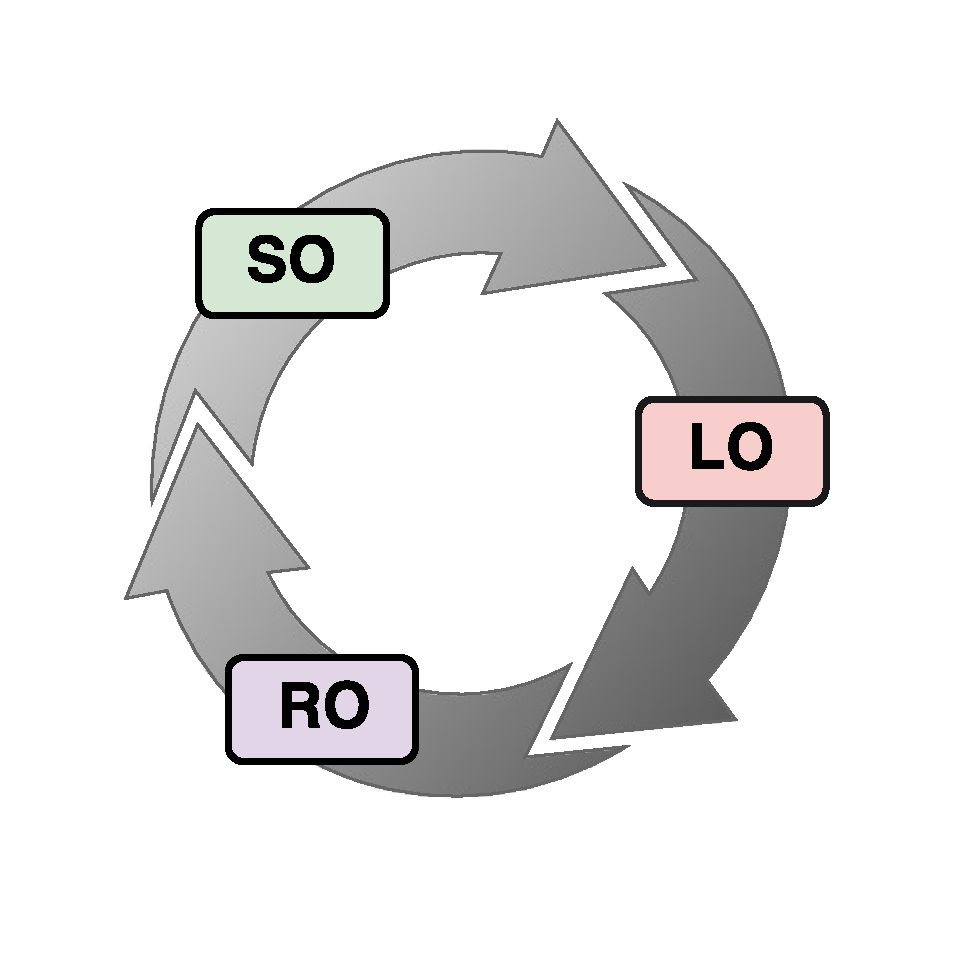
\includegraphics[scale=.35]{Figures/04_NSO/fun_orch}
    \caption{Different orchestrator functions: Resource Orchestration, Service Orchestration, and Lifecycle Orchestration. There is a relationship of dependency and continuity between the functions.}
    \label{funOrch}
\end{figure}

The Service Orchestration is responsible for service composition and decomposition. It can be taken as the upper layer, focused on the interaction with other components such as Marketplace and \gls{oss} / \gls{bss}. The Lifecycle Orchestration deals with the management of workflows, processes, and dependencies across service components. Besides, it maintains the services running according to the contracted Service Level Agreement. Finally, the Resource Orchestration is in charge of mapping service requests to resources, either virtual and/or physical. This mapping occurs across elements such as \gls{nfvo}, \gls{ems}, and \gls{sdn} controllers.


To accomplish this, the orchestrator may be inserted in each layer of telecommunication network stack, from the application layer down to the data plane. Therefore, different orchestrators can exist in each plane, not being limited to a single orchestrator~\cite{Alvizu2016AdvanceEra}. Some of the existing orchestration solutions use an orchestrator logically centralized and consider only ``softwarized'' networks (see Section~\ref{sec:proj}). However, this is very challenging for large and heterogeneous networks. 

Lifecycle is used to manage a network service with various states (created, provisioned, scaled, stopped, etc.). When some action is applied to a network service (e.g., provision a network service), many activities may be needed to apply to the components of this network service. Hence, a workflow is used to execute a bunch of tasks in the correct order. Each state of lifecycle can generate one or more activities on workflows. The Figure~\ref{fig:lifeWork} depicts the relationship between lifecycle and workflow of a Network Service. 

Figure~\ref{fig:lifeWork2} presents an example to improve the real definition of lifecycle and workflow in the context of network service. One of the states in the service lifecycle is the \textit{Created}. In order to achieve such state is necessary to execute four tasks: create \gls{vdu}1, create \gls{vdu}2, configure network and run the application. Therefore, the state only is changed from creating to created when all those activities are completed.

\begin{figure*}[thpb]
\centering
 \subfigure[]{
   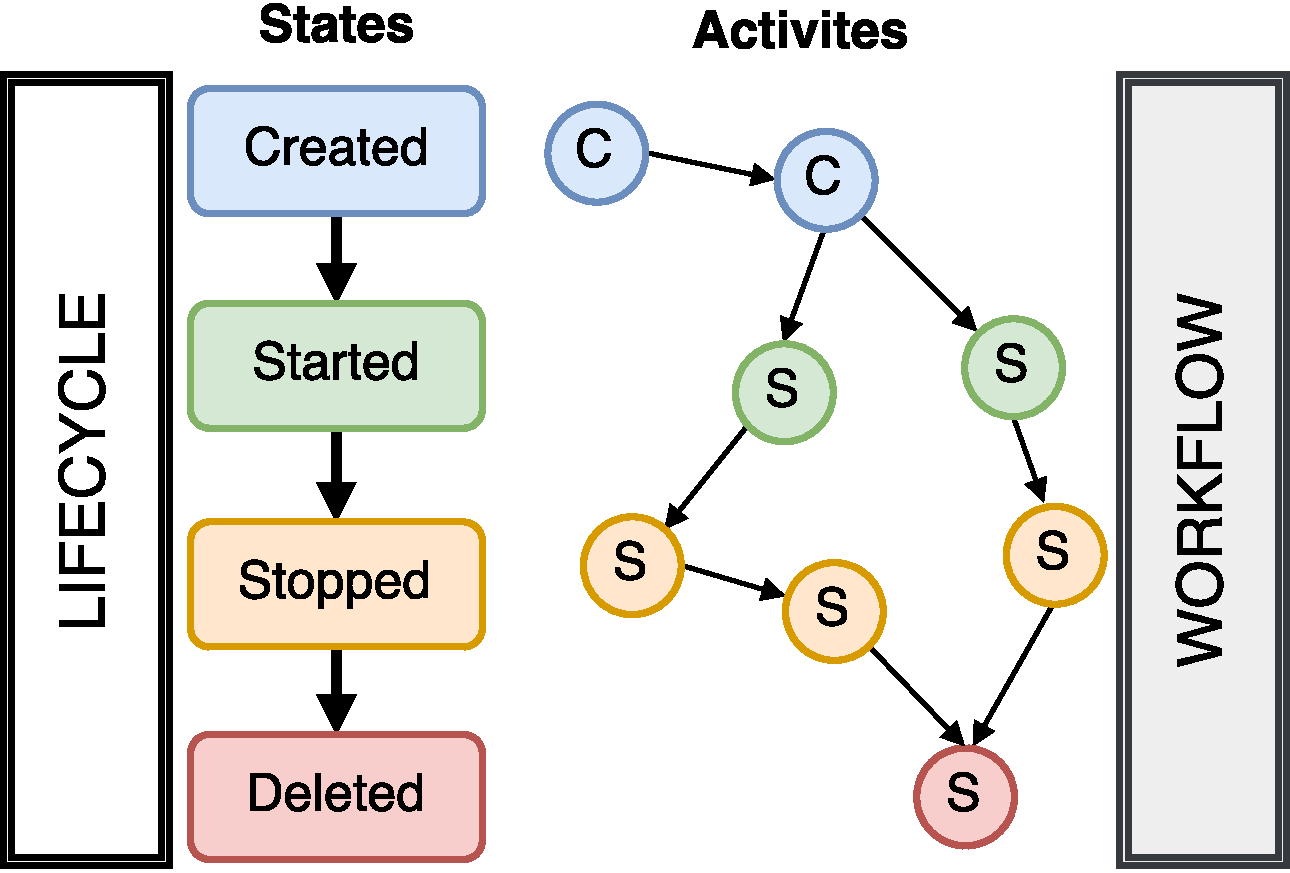
\includegraphics[scale=.3]{Figures/04_NSO/life_work}
   \label{fig:lifeWork}
 }
 \subfigure[]{
   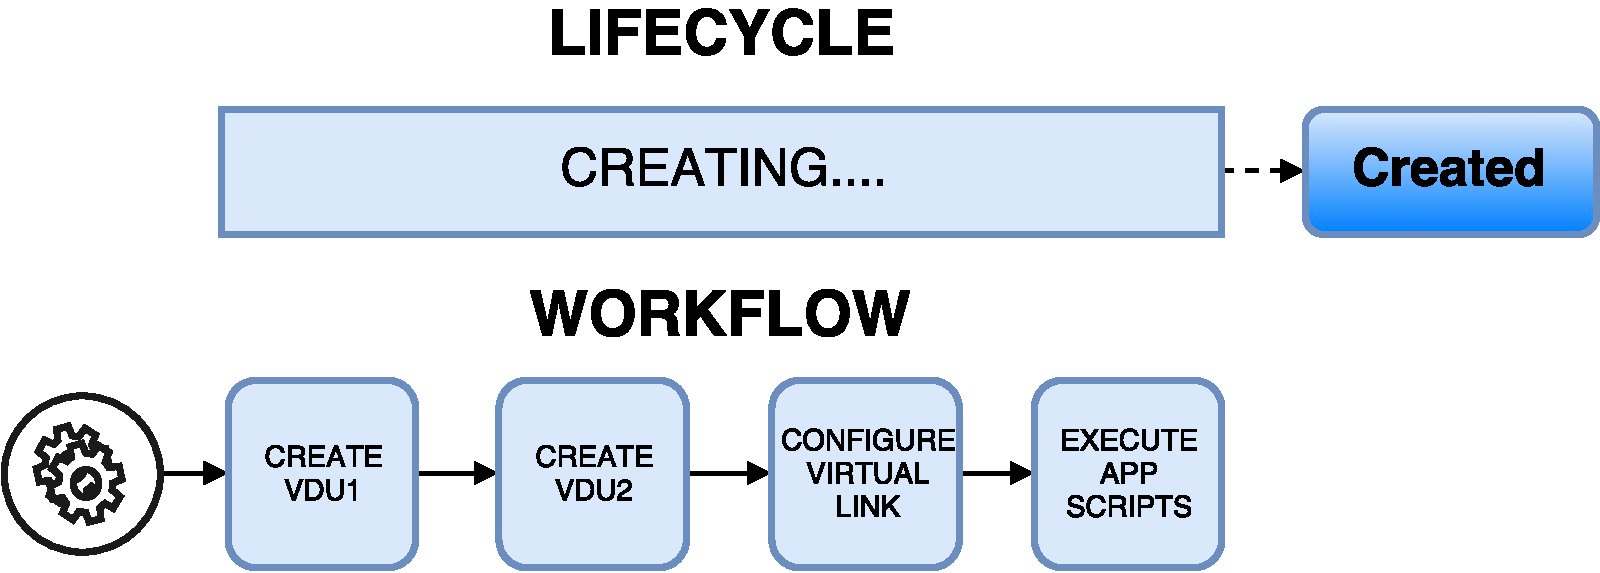
\includegraphics[scale=.3]{Figures/04_NSO/life_work2} 
   \label{fig:lifeWork2}
 }    
 \caption{Difference between Lifecycle and Workflow: (a) Lifecycle -- sequence of states and workflow -- activities in correct order and (b) example of network service lifecycle.}
 \label{fig:lifeworkflow}  
\end{figure*}

Service lifecycle automation will allow that requested service remains in a desired state of behavior during its lifetime. With the automation, the system responds proactively to changes network and service conditions without human intervention, getting resilience and faults tolerance. These functional aspects of an orchestrator to guarantee the state of a network towards a service goal are also being referred to as Intent-based Networking (IBN), cf.~\cite{ibn}.

We refer to the \acrfull{nso} when applied in the services deployment performed by telecommunication operators and service providers. We regard NSO not precisely as a unique technology but as a concept to  understand network services in detail, relying on multiple technologies and paradigms to achieve such an overarching goal. In a nutshell, network service orchestration comprises the semantics of requested service, and thereby it coordinates specific actions in order to fulfill the service requirements and to manage its end-to-end lifecycle. 

%Network service orchestration is one of the functions of the orchestrator defined by \gls{etsi} \gls{nfvmano} (more details in Section~\ref{subsec:func}). However, in our proposal, the definition of \gls{nso} is more comprehensive. Therefore, Network Service Orchestration comprises understanding the semantics of requested service in order to coordinate the specific actions to fulfill service requests and states management. 

%meanings and relations

%In addition, it overcomes the technological and administrative domains boundaries towards deploying the end-to-end services. 

The entire orchestration process proposed by NSO involves business and operations that go beyond the delivery of \textit{network services} as defined by \gls{etsi}. \gls{etsi} \gls{nfvmano} is a platform for management and orchestration required to provisioning \glspl{vnf} in an \gls{nfv} domain. The \gls{mano} is agnostic and thus has no insight of what is executed within a \gls{vnf}, restricting its responsibility and capability to the VNF instantiation and lifecycle management.

Based on Figure~\ref{mdo}, the \gls{mdo} understands the operating capabilities of the \gls{ns} in a broad sense. When a customer demands an \gls{ns}, firstly it requests the order to a service provider or telecommunication operator through Business-to-Business (B2B) interface or a trading platform we refer to as Marketplace. After that, the \gls{mdo} interacts with any \gls{mano} element or other elements (e.g., OSS/BSS, SDN Controllers, Analytic Systems)  to create the \gls{ns}. Therefore, a given MANO does not know if the VNFs it is deploying is a load balancer, firewall, or gateway. Meanwhile, the \gls{do} just coordinates and manages the orchestration process at a given domain, connecting the involved elements such as network systems, SDN controllers, management software, and IT software platforms.

%The \gls{nso} understands the operating capabilities of the \gls{ns} broadly. When an \gls{ns} requires being created, the \gls{nso} interacts with the \gls{mano} or other elements to request the creation of the service. The \gls{mano} doesn't know if the \glspl{vnf} it is deploying is a load balancer, firewall or gateway. The \gls{nso} coordinates and manages the orchestration process, connecting the involved elements such as network systems, controllers, management software, and telecommunications IT software platforms. 



In this sense, different organizations and telecommunication enterprises have developed many open source projects, driving orchestration evolution towards open standards that it will permit the implementation of products with a large scale of integration. Section~\ref{sec:proj} addresses some of these projects.

In addition, the customers are demanding full information regarding a given hired network service such as detailed pricing, real-time analytics, and a precise control over the service. NSO can offer more information to the customers and put more control into their hand. Its objective is to understand the service profoundly and to enable that providers/operators attend customer demands. 

From an operator and service provider viewpoint, NSO enables to set up new end-to-end services in minutes, keeping those services working and ensuring acceptable performance levels. This process reduces OPEX and provides enhanced services creating new market opportunities and raising the revenues.  It opens up chances for different companies to become service providers or provide virtual network functions, as well.
%On the customer's side, \gls{nso} provides detailed information regarding a given hired network service to its customers, since they demand detailed pricing, real-time analytics, and control over requested service. On the other hand, provider/operators promise customers to set up new end-to-end services in minutes, keeping those services working and ensuring acceptable performance levels. Thus, the \gls{nso} will create new opportunities for companies to become service providers or to provide virtual network functions. 

%In short, given its supportive technologies (SDN, NFV, and Cloud Computing), 
%\gls{nso} intends to increase service agility and operational efficiency while speeding up new service delivery with reduced costs. 

% \gls{nso} is in charge of all network service lifecycle and delivers an end-to-end connectivity service. To achieve so, orchestration is supported by advances in cloud computing, and technologies such as \gls{sdn} and \gls{nfv}, which offer the ability to reconfigure the network quickly as well as programming the forwarding and processing of the traffic. Figure~\ref{nso_rel} aims at illustrating the relationships between \gls{nso}, \gls{nfv}, \gls{sdn}, and Cloud Computing.

% \begin{figure}[t]
%   \centering
%   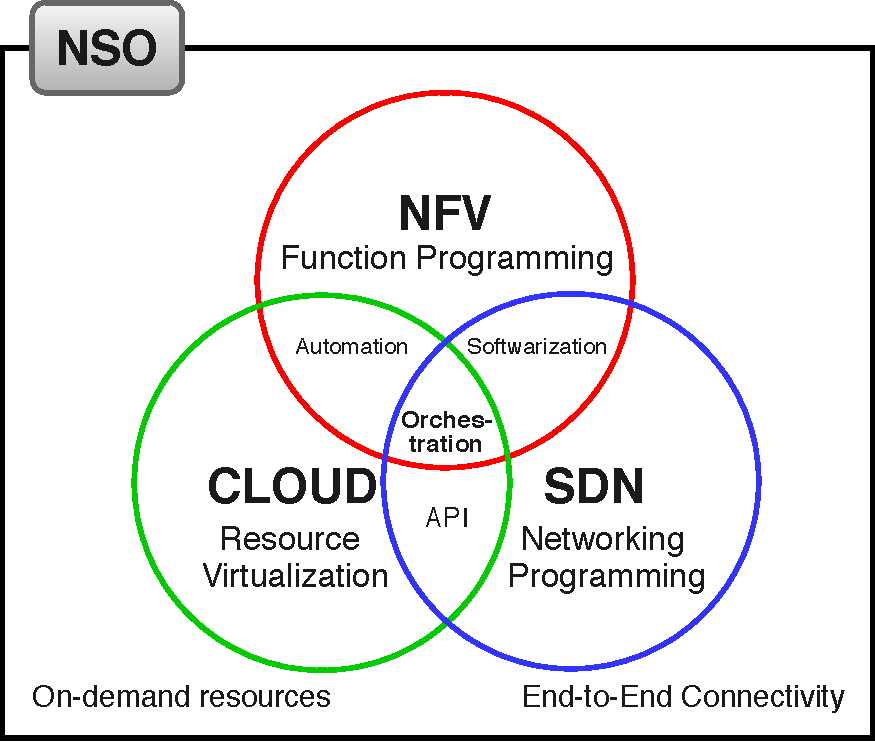
\includegraphics[scale=.4]{Figures/04_NSO/nso_rel}
%     \caption{Illustration of relationships between \gls{nso}, \gls{nfv}, \gls{sdn}, and Cloud.}
%     \label{nso_rel}
% \end{figure}

% Each one of these paradigms has different functions: high level orchestration for \gls{nso}, function programming for \gls{nfv}, networking programming for \gls{sdn},  and resource virtualization for cloud computing. They can work in an integrated pattern to offer advantages such as agility, cost reduction, automation, softwarization and end-to-end connectivity, to enable novel services and applications such as 5G networks.

%After this analysis, we can identify the main NSO features: (i) high-level vision of the \gls{ns}, (ii) smart services deployment and provisioning, (iii) single and multi-domain environment support, (iv) interaction with different MANO and non-MANO elements. %In our vision, NSO is not precisely a technology but a concept that understand network services in detail and uses existing technologies and paradigms to achieve such goal.

After this analysis, we can identify the main NSO characteristics as follows: 
\begin{itemize}
\item \textit{High-level vision of the \gls{ns}} that permit an overview of all involved domains, technological and administrative. 
\item \textit{Smart services deployment and provisioning}. These are related to in-deep knowledge about the services, what enable better make decisions. 
\item \textit{Single and multi-domain environment support} that provide deployment of end-to-end service independently of geographical location.
\item \textit{Proper interaction with different MANO and non-MANO elements} which leads to better-executed workflows.
\item \textit{Fulfilling new market opportunities}, offering enhanced services and reducing OPEX.    
\end{itemize}

%\subsection{Orchestrator Functions}
%\label{subsec:func}

%%%%%% Section~\ref{sec:def} identifies the various areas of term orchestration. Orchestration can be inserted in the context of cloud, \gls{nfv}, management systems, web services and more recently in the deployment of end-to-end network service in large networks with multiple technologies and administrative domains. In this scope, the orchestrator is the component responsible for automatic resource coordination and control, as well as service provision to customers. 

%In the network service domain, the exact definitions of the roles of the Orchestrator is open issue  \cite{Alvizu2016AdvanceEra}.



%Besides providing an interaction with other elements, the orchestrator abstracts physical and virtual resources, transparently exposing them to service providers as Google, Amazon, and Microsoft. It gives service providers further control of their network services and enables developers to create new services and functions.


%%%%%% INSERTED SECTION 3A %%%%%%%

% To accomplish this, the orchestrator may be inserted in each layer of telecommunication network stack, from the application layer down to the data plane. Therefore, different orchestrators can exist in each plane, not being limited to a single orchestrator~\cite{Alvizu2016AdvanceEra}. Some of the existing orchestration solutions use an orchestrator logically centralized and consider only ``softwarized'' networks (see Section~\ref{sec:proj}). However, this is impracticable for large and heterogeneous networks. 

% Lifecycle is used to manage a network service with various states (created, provisioned, scaled, stopped, etc.). When some action is applied to a network service (e.g., provision a network service), many activities may be needed to apply on the components of this network service. Hence, a workflow is used to execute a bunch of tasks in correct order. Each state of lifecycle can generate one or more activities on workflows. The Figure~\ref{fig:lifeWork} depicts the relationship between lifecycle and workflow of a Network Service. 

% Figure~\ref{fig:lifeWork2} presents an example to improve the real definition of lifecycle and workflow in the context of network service. One of the states in the service lifecycle is the \textit{Created}. In order to achieve such state is necessary to execute four tasks: create \gls{vdu}1, create \gls{vdu}2, configure network and run the application. Therefore, the state only is changed from creating to created when all those activities are completed.

% \begin{figure*}[thpb]
% \centering
%  \subfigure[]{
%    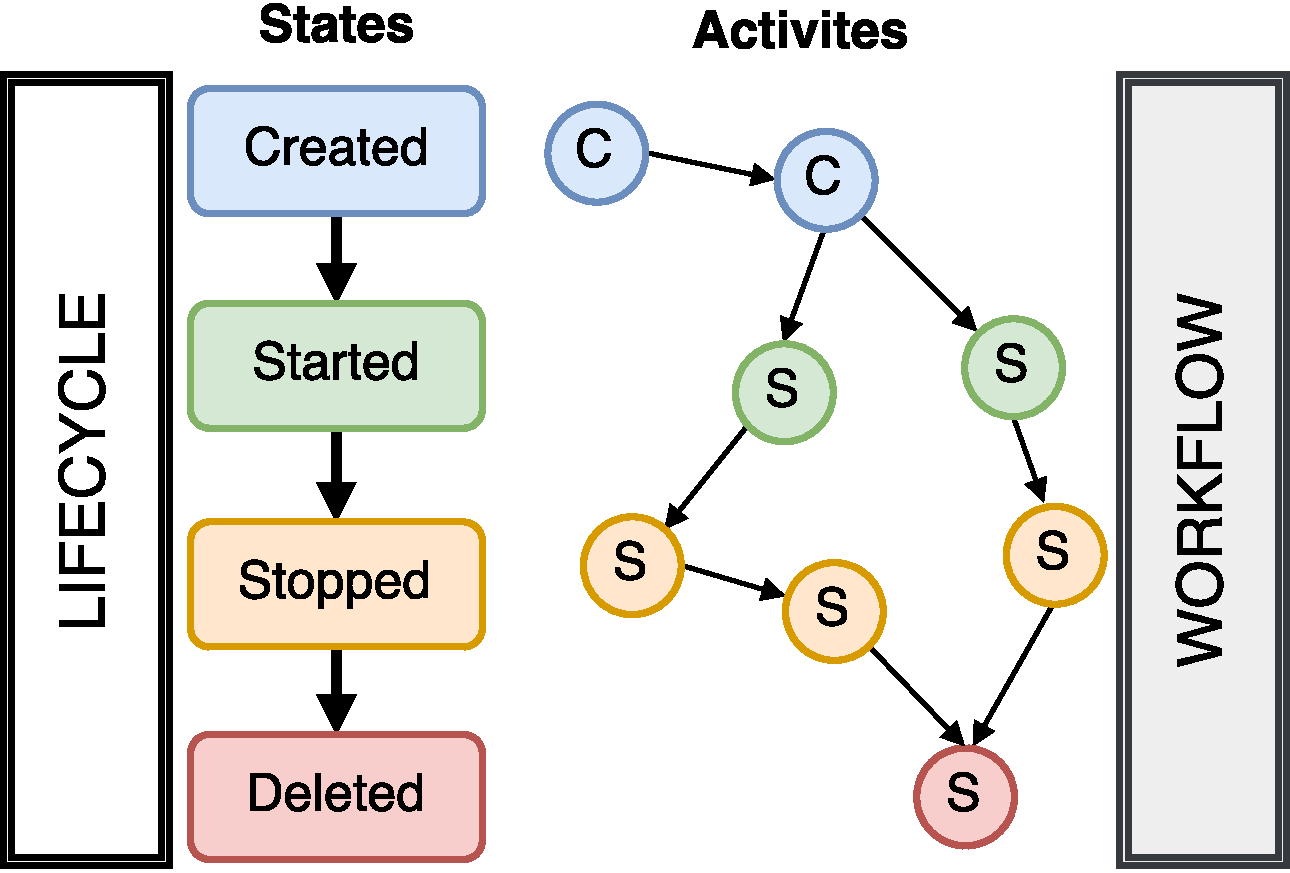
\includegraphics[scale=.3]{Figures/04_NSO/life_work}
%    \label{fig:lifeWork}
%  }
%  \subfigure[]{
%    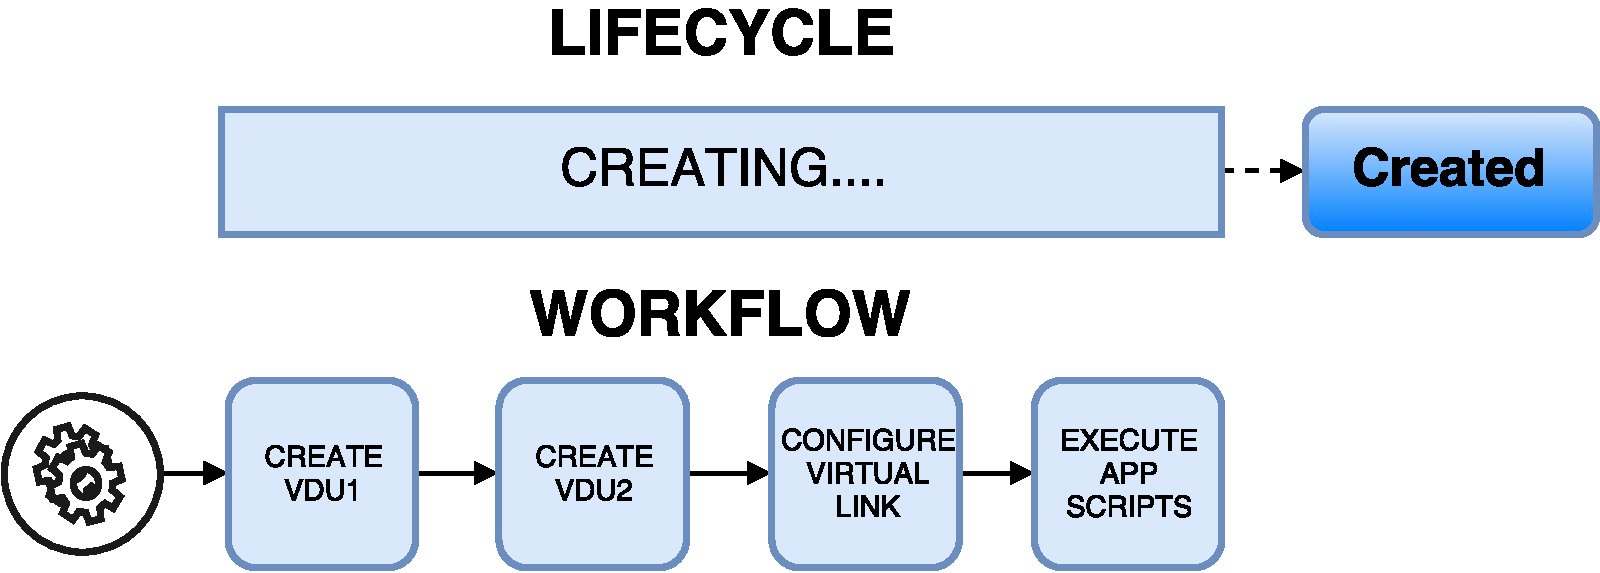
\includegraphics[scale=.3]{Figures/04_NSO/life_work2} 
%    \label{fig:lifeWork2}
%  }    
%  \caption{Difference between Lifecycle and Workflow: (a) Lifecycle -- sequence of states and workflow -- activities in correct order and (b) example of network service lifecycle.}
%  \label{fig:lifeworkflow}  
% \end{figure*}

% Service lifecycle automation will allow that requested service remains in a desired state of behavior during its lifetime. With the automation, the system responds proactively to changes network and service conditions without human intervention, getting resilience and faults tolerance. These functional aspects of an orchestrator to guarantee the state of a network towards a service goal are also being referred to as Intent-based Networking (IBN), cf.~\cite{ibn}.

%%%%%% INSERTED IN SECTION 3A %%%%%%

%%% CH this final sentence does not add much:
%The orchestration is a central theme of the current telecommunication operators and service providers conversation about the future networks. Note that the orchestrator has a crucial function in this scenario. Based on Figure~\ref{mdo}, the NSO function can be performed by a \acrlong{mdo}. It is worth mentioning that \gls{mdo} can be implemented in one or more components. Next, we define aspects and concepts towards a classification of NSO approaches.


%In last years, many orchestration solutions have been created, but they have limitations yet (see Section~\ref{sec:proj}).

%The success of a service orchestrator depends on its ability to measure the network performance, to assess service quality using a small set of metrics and to provide network diagnosis and root cause analysis during service disruptions. In parallel, the orchestrator must support network resource scheduling which can adapt to near real-time service demands.\cite{c5}%reescrever

%Up to date, the impression is that even very evolved and complex controllers such as ONOS and OpenDaylight have not reached yet a very stable stage of development, and thus a lot has to be implemented in the orchestrator to customize it to the operators’ needs \cite{c35}.%reescrever

%service providers quickly add features and drive down operations costs.


\subsection{Single and Multi-Domain Orchestration}
\label{sec:domain}

The \gls{nso} works at a higher level in the control and management stack with interfaces to the OSS/BSS. During a network service creation, the orchestration process can exceed the domains boundaries being necessary to use resources and/or services of other providers or operators. Such resources comprising physical and virtual components. Thus, the \gls{nso} is supposed to provide service delivery both within single and/or multi-domain environments.

Orchestration in the single and multi-domain environment is different. In a single domain, the orchestrator is in charge of all services and resource availability within its domain as well as has total control over those resources. A domain orchestrator manages the network service lifecycle and interacts with other components not only to control \glspl{vnf}, but also computing, storage, and networking resources. Its scope is limited by administrative boundaries of the provider. As shown in Figure~\ref{mdo}, domain orchestrators can orchestrate heterogeneous technological domains such as \gls{sdn}, \gls{nfv}, Legacy, and Data center. Under a single domain environment, it is noticeable that the domain orchestrator works as described by \gls{etsi} in \cite{ETSIIndustrySpecificationGroupISGNFV2014NetworkOptions}. 

On the other hand, in a multi-domain environment,  local orchestrators do not know the resources and topologies used by other providers. So, multi-domain orchestration is more complex, since it is supposed to provide end-to-end services, which requires cross-domain information exchange features (cf.~\cite{md2}). %This exchange has to be standardized. 
Currently, there is not a standard for information exchange process in multi-domain environments, either multi-technology domains or multiple administrative domains. There are some multi-domain orchestration candidates, e.g., T-NOVA FP7 project \cite{FP7projectT-NOVAT-NOVAInfrastructures}, ONAP~\cite{onap}, Escape \cite{Sonkoly2015Multi-DomainClouds}, and \gls{5gex} \cite{Bernardos20155GInfrastructures}. All of them will be discussed later in this survey.

%There are many different mappings between administrative, technology and tenant domains but is out of scope for the present article. %ETSI
\gls{etsi} proposes some options regarding multi-domain orchestration. Initially, \gls{etsi} \gls{nfv}  Release 2 presents two architectures to address multi-domain scenarios~\cite{ETSIIndustrySpecificationGroupISGNFV2014NetworkOptions}. In the first, the \gls{nfvo} is split into \textit{Network Service Orchestrator}, manages the network service, and \textit{Resource Orchestrator}, provides an abstract resource present in the administrative domain. A use case for this first option is illustrated in Figure~\ref{fig:use1}. A Network Operator offers resources to different departments within the same operator, likewise to a different network operator. One or more Data centers and \glspl{vim} represent an administrative domain and provide an abstracted view of its resources (virtual and physical). The Service Orchestrator and VNF Manager can or can not be part of another domain. In this use case, service can run on the infrastructure provided and managed by another Service Provider.
% First approach of shared infrastructure using multiple administrative domains.

The second architecture does not split the \gls{nfvo}, but creates a new reference point between NFVOs (See Figure~\ref{fig:use2}) called  Umbrella \gls{nfvo}. This use case requires the composition of services towards deploying a high-level network service. Such service can include network services hosted and offered by different administrative domains. Each domain is responsible for orchestrating its resources and network services. This approach has objectives similar to first, however, an administrative domain is also composed of \glspl{vnfm} (together with their related \glspl{vnf}) and \gls{nfvo}. The \gls{nfvo} provides standard \gls{nfvo} functionalities, with a scope limited to the network services, \glspl{vnf} and resources that are part of its domain.
% Second approach of shared network services using multiple administrative domains.

More recently, the \gls{etsi} \gls{nfv} Release 3 presented others options to support network services across multiple administrative domains~\cite{ETSIGRDomains}. In particular, the use case entitled ``Network Services provided using multiple administrative domains" proposes a multi-domain architecture using \gls{nfvmano}. Such architecture introduces the new reference point named ``Or-Or" between \glspl{nfvo} to enable communication and interoperability. Differently of the second option (Figure~\ref{fig:use2}), in this approach, there is a hierarchy between the domains. In the example shown in Figure~\ref{fig:use3}, \gls{nfvo} in Administrative Domain C is on-top, using network services offered by Administrative Domains A and B, as well as managing composite \gls{ns} lifecycle.    

\begin{figure*}[t!]
\centering
 \subfigure[]{
   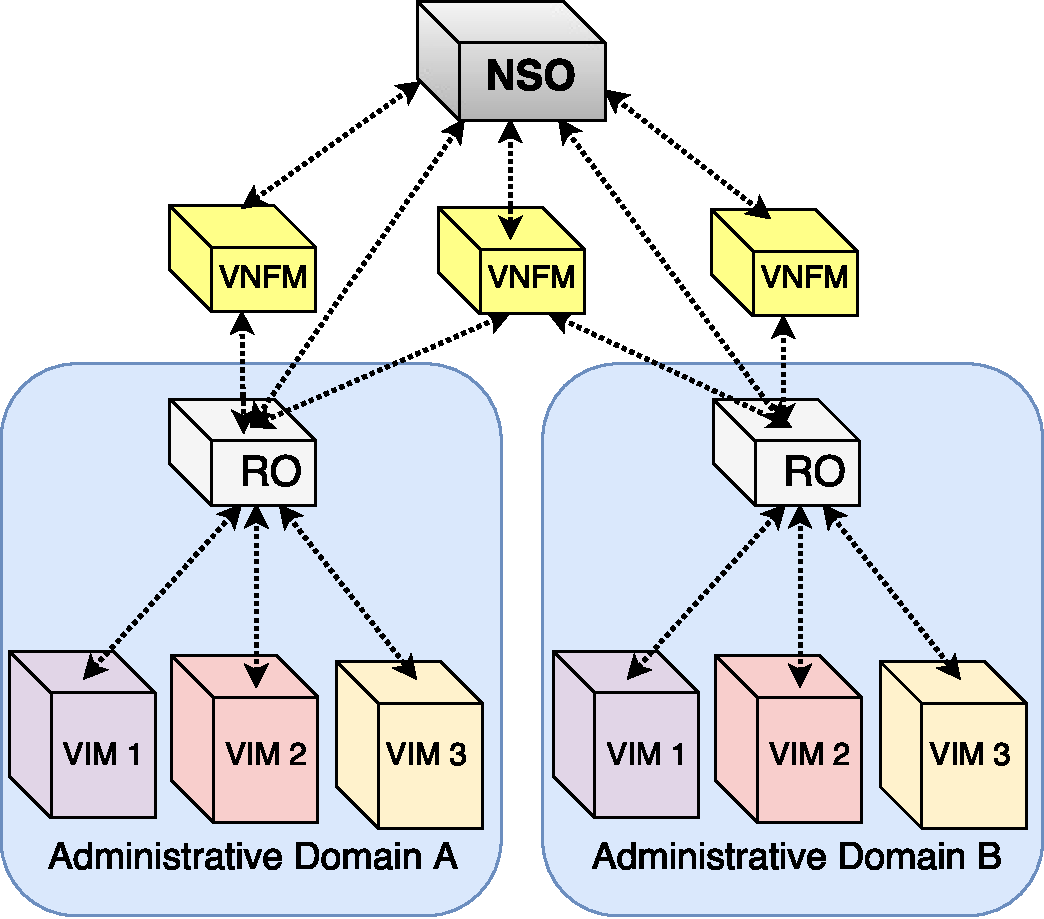
\includegraphics[scale=.31]{Figures/04_NSO/mdo_etsi_1}
   \label{fig:use1}
 }
 \subfigure[]{
   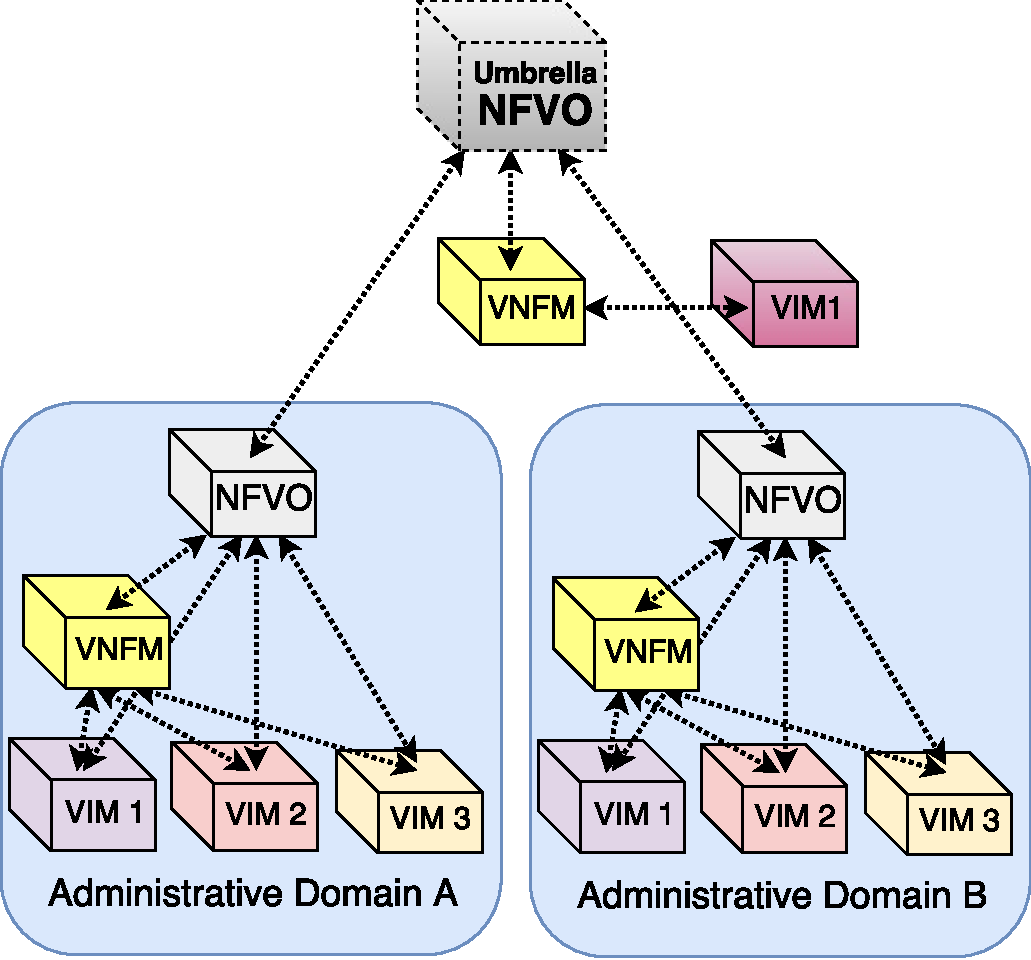
\includegraphics[scale=.31]{Figures/04_NSO/mdo_etsi_2} 
   \label{fig:use2}
 }
 \subfigure[]{
   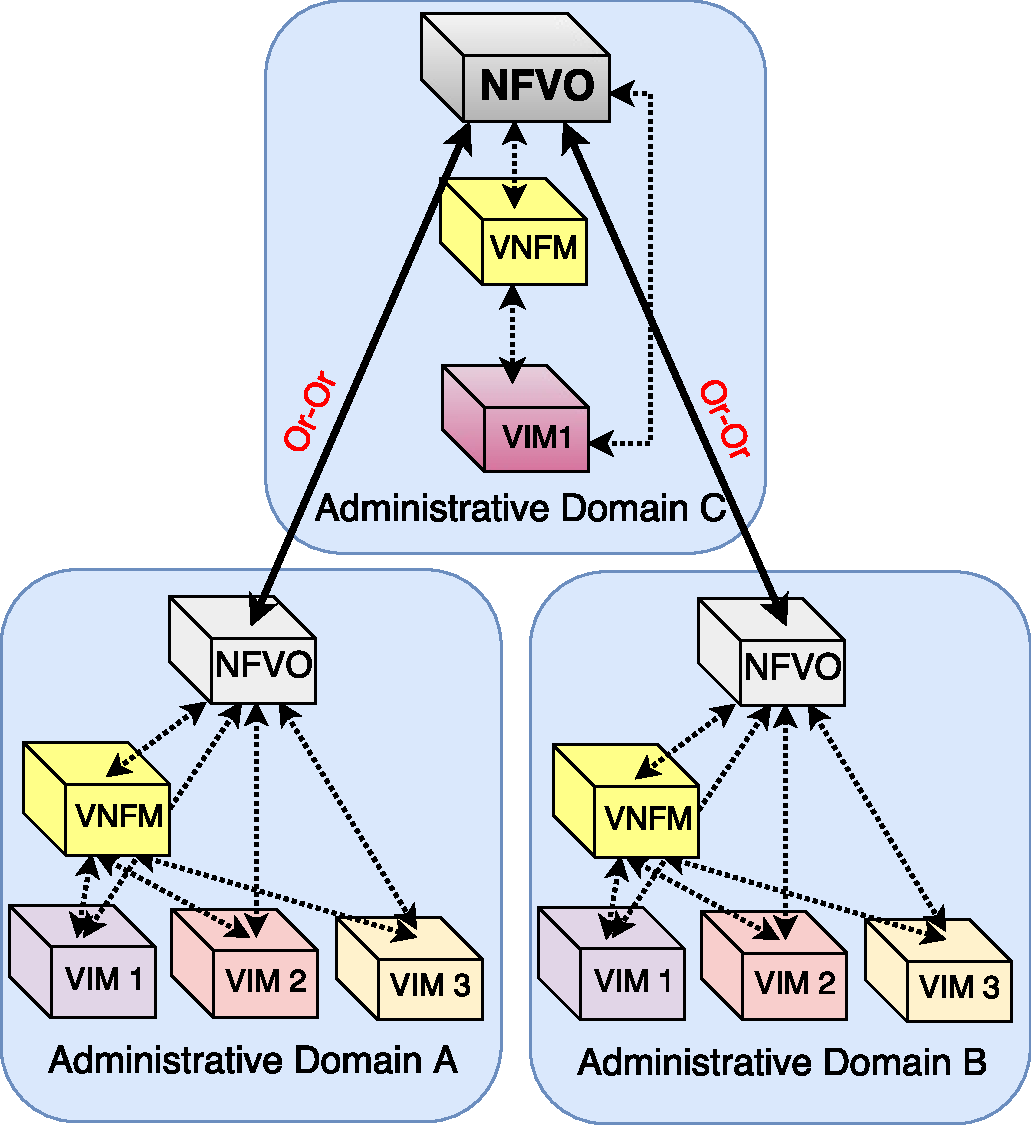
\includegraphics[scale=.31]{Figures/04_NSO/mdo_etsi_3} 
   \label{fig:use3}
 }
 \caption{\gls{etsi} approaches for multiple administrative domains: (a) approach in which the orchestrator is split into two components (NSO and RO), (b) approach with multiple orchestrators and a new reference point: Umbrella NFVO, (c) approach that introduces hierarchy and the new reference point Or-Or. Adapted from~\cite{ETSIIndustrySpecificationGroupISGNFV2014NetworkOptions} and~\cite{ETSIGRDomains}.}
 \label{fig:k-clique}  
\end{figure*}

In the scope of this paper, end-to-end network services are composed of one or more network functions interconnected by forwarding graphs. Such services might span multiple clouds and geographical locations. Given that, they require complex workflow management, coordination, and synchronization between multiple involved domains (infrastructure entities), which are performed by one (or more) orchestrator(s). Examples of end-to-end services are virtual extensible LAN (VxLAN), video service delivery, and virtual private network.

%\subsection{Definition NSO}

%%%%%%%%%%%%%%%%%%%%%%%%%%%%%%%%%%%%%
%The NSO provides the network services decoupling from specific network components, while automatically configuring the service from a vision more complete of the resources.    

%Network Service Orchestration aims to manage and orchestrate services comprised of physical and virtual resources across multiple technology and vendor domains. Beside it provides orchestration and management integration among network systems, management software, and telecommunications IT software platforms. 

%This can enable real-time automation, monitoring, and service assurance for a wide range of network-based services.

%NSO is an agile approach to streamlining and automating the service lifecycle in a sustainable fashion for coordinated management and control across all network domains responsible for delivering an end-to-end Connectivity Service.

%Multi-domain service orchestration helps aspect of access to everything, at any time, from any location, which is escalating performance, availability, and bandwidth demands that service providers and network operators are wishing.


\subsection{Taxonomy}

While many aspects of orchestration are under active development and commercial roll-outs, others are still in a preliminary maturity phase. This subsection enumerates central concepts and characteristics related to any NSO approach. It becomes very challenging trying to summarize all concepts related to orchestration in a single work, a challenge exacerbated by the fast-evolving pace of so many moving pieces, from standards to enabling technologies. Figure~\ref{tax} presents the proposed taxonomy as the result of extensive literature research as well as practical experiences with a number of orchestration platforms and research projects.   

\begin{figure*}[thpb]
  \centering
  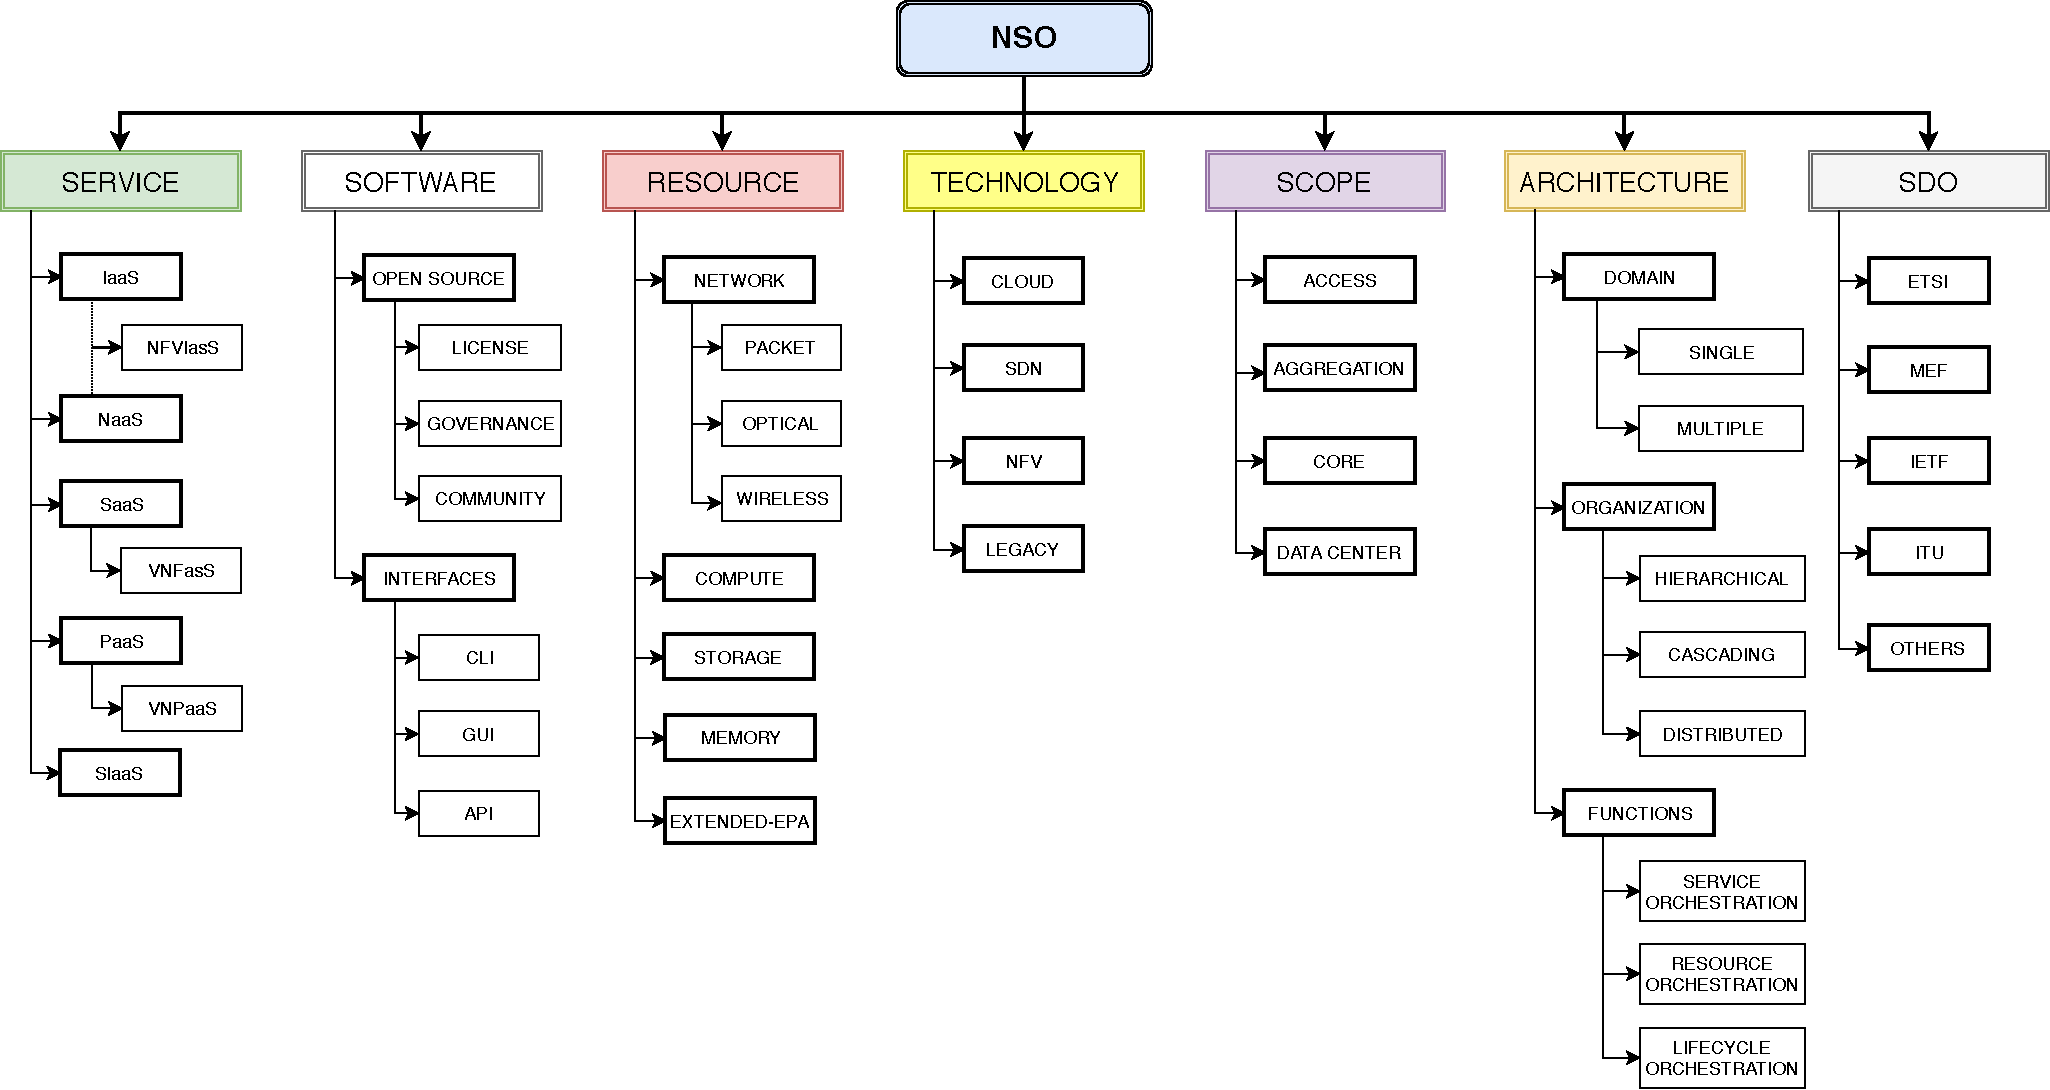
\includegraphics[scale=.51]{Figures/04_NSO/taxonomy}
    \caption{\gls{nso} Taxonomy with seven approach: Service Model, Software, Resource, Technology, Scope of Application, Architecture, and Standards \acrfull{sdo}.}
    \label{tax}
\end{figure*}

We identify seven key aspects to characterize network service orchestration: 
\begin{enumerate}
\item \textit{\textbf{Service} Models}. Relates to the type of services unlocked by the \gls{nso}, which may offer new business and relationships and opportunities  (e.g., \gls{vnfaas}, \gls{slaas}).
\item \textbf{\textit{Software}}: Identifies major software-related characteristics of the orchestration solutions, including specificities of the  management and standard interfaces.
\item \textbf{\textit{Resource}}: Refers to the type of underlying resources (e.g., network, compute, and storage) used for the network service deployment.
\item \textbf{\textit{Technology}}: Points to target technologies for \gls{nso} (e.g., Cloud, \gls{sdn}, \gls{nfv}, and Legacy).
\item \textit{\textbf{Scope}}: Considers the application domain in terms of network segments embraced by the network service orchestration (i.e., from access network to data centers).  
\item \textbf{\textit{Architecture}}: Unfolds into three relevant architectural dimensions with relate to single- and multi-domain orchestration and functional  organization.
\item \textit{\textbf{SDO} (Standards Development Organization)}: Relates to standardization activities in scope of the NSO.
\end{enumerate}

Additional sub-areas contribute to an in-depth analysis in different contexts, which are  further  discussed in the following sections. 

\subsubsection{Service Models}
This aspect corresponds to the different service models related to orchestration process. Each service is inserted in the context of cloud, \gls{sdn}, and/or \gls{nfv}. Cloud computing offers three categories of services such as \gls{iaas}, \gls{paas} and \gls{saas} \cite{Leavitt2009}. In \gls{iaas}, Cloud Service Provider (CSP) renders a virtual infrastructure to the customers. In \gls{paas}, CSPs provide development environment as a service. Finally, \gls{saas} is a service that furnishes applications hosted and managed in the cloud. 

\gls{sdn} and \gls{naas} paradigms can be gathered to provide end-to-end service provisioning. While SDN supply the orchestration of underlying network (switches, router, and links), the \gls{naas} is responsible for private access to the network and customer security~\cite{Karakus2017QualitySurvey}. 

The \gls{nfv}, in turn, can offer new services including \gls{nfviaas}, \gls{vnfaas}, \gls{slaas} and \gls{vnpaas}. The \gls{nfviaas} provides jointly \gls{iaas} and \gls{naas} tailored for \gls{nfv}. \gls{vnfaas} is a service that implements virtualized Network Functions to the Enterprises and/or end customers. \gls{vnpaas} is a platform available by service providers allowing customers to create their own network services. The \gls{slaas} is a concept that the slices are traded and used to build infrastructure services.

All these services can work in parallel to offer higher-level services. Each one acts in a specific area and offers features to customers, enterprises, or other providers.   

\subsubsection{Software} 
There are many software artifacts related to orchestration covering from a single cloud environment up to more complex scenarios involving multi-domain orchestration. These solutions are outcomes of open source initiatives, research projects or commercial vendors.   

Open source approaches significantly accelerate consensus, delivering high performance, peer-reviewed code that forms a basis for an ecosystem of solutions. Open source makes it possible to create a single unified orchestration abstraction.  Thus, both research projects and commercial vendors leverage open source technologies to accelerate and improve their solutions. Operators, such as Telefonica, China Mobile, AT\&T, and NTT, appear committed to using open source as a way to speed up their development of orchestration platforms~\cite{Sdxcentral20162016:}.

The \gls{osi}\footnote{http://opensource.org} defines licenses under Open Source Definition compliance, which allows code and software to be freely used, shared and modified. The more popular open source licenses are Apache License 2.0, \gls{bsd}, GNU General Public License (GPL), Mozilla Public License 2.0, and Eclipse Public License. Namely, the most important orchestration projects and frameworks (for instance, Aria, Cloudify, CORD, Gohan, Open Baton, Tacker, ONAP, SONATA, and T-NOVA) present a widespread usage of Apache License 2.0.

Another topic related to open source is governance. In short, governance defines the processes, structures, and organizations. It determines how power is exercised and distributed and how decisions are taken. Commonly, a governing board is responsible for the budget, trademark/legal, marketing, compliance, and overall direction, while a technical steering committee is responsible for technical guidance. 

An open source orchestration project may be organized as a single community (e.g., vendor-lead) or can be hosted (and eventually integrated with other projects) by a foundation entity~\cite{Opensource.comFourOpensource.com}. A remarkable example is the Linux Foundation, which among multiple networking related projects is in charge of  ONAP, an open source platform aiming at the automation, design, orchestration, and management of SDN and NFV services. Another noteworthy example of an orchestration open source project under the Linux Foundation flagship aiming at delivering a standard \gls{nfv}/\gls{sdn} platform for the industry is Open Platform for NFV (OPNFV)~\cite{LinuxFoundation}.

NSO solutions need to perform management tasks such as remote device configuration, monitoring and fault management. Moreover, they require defining an interface of communication between various software components. For this, there are diverse types of management and  standard interfaces such as \gls{cli}, \gls{api}, and \gls{gui}. The \gls{cli} just is used to execute commands directly in the software using remote access via SSH or Telnet. The \gls{api} enables the remote management and interconnection with other softwares through specifics commands. The majority of solutions use REST-based \gls{api}. \gls{gui}, in turn, offers a graphic interface that makes it easier its use.   

\subsubsection{Resource}
During the creation of a network service, the resource orchestration is responsible for orchestrating the underlying infrastructure. Such infrastructure is composed of heterogeneous hardware and software, and different features for hosting and connecting the network services. The resources include compute, storage, network~\cite{Ordonez-Lucena2017NetworkChallenges}, memory, and Extended-\gls{epa}. 

Regarding network, there are three types: packet, optical and wireless (e.g., Wi-Fi, wi-max, and mobile network). Compute, storage, and memory are resources shared among a multitude of network services.  

Resources are shared and abstracted making use of virtualization techniques (e.g., para-virtualization~\cite{4299349}, full virtualization~\cite{4482796}, and containers~\cite{6906035}), defining virtual infrastructures that can be used as physical ones.
For an \gls{nso} solution to be suitable, its virtualized functions must deliver near native (i.e., non-virtualized) performance. For that, EPA capabilities need to be implemented and extended in underlying platform providing highly performant and efficient system. Some examples are (i)\textit{~\gls{numa}}, divide the memory into zones, which are allocated to specific CPUs, (ii) \textit{CPU pinning}, run a particular virtual function’s virtual CPU on a specific physical CPU, (iii)~\textit{\gls{dpdk}}, libraries to accelerate packet processing workloads, and (iv) \textit{Native P4 enabled switches}, provide to programmable pipeline and high-performance forwarding. 

%%%%%% Sharing and management of resources are much more complex in multi-domain scenarios. The NSO needs to know all the available resources towards the efficient deployment of the \glspl{ns}. %%%%%% 

%In multi-domain scenarios In the NFV architecture, the \gls{nfvi} is associated with the virtualization of the compute, network, and storage resources. 

\subsubsection{Technology}
NSO involves complex workflows and different technologies involved throughout orchestration process: cloud computing, \gls{sdn}, \gls{nfv}, and legacy.      

The cloud computing paradigm provides resource virtualization and improves resource availability and usage by means of orchestration and management procedures. This includes automatic instantiation, migration, and snapshot of \glspl{vm}, High-Availability, and dynamic allocation of resources~\cite{ETSI2012NetworkAction}. 

The \gls{sdn} promotes control across network layers and logical centralization of network infrastructure management. Its main functions is to connect the \glspl{vnf} and the \gls{nfvi}-\glspl{pop}. In parallel, the \gls{nfv} technology promotes the network functions programming in order to enable elasticity, automation, and resilience in cloud environments \cite{Rotsos2017NetworkSurvey}. As illustrated in Figure~\ref{nso_rel}, cloud computing, \gls{sdn} and \gls{nfv} are enabler technologies to the \gls{nso}. The NSO must also handle legacy technologies such as MPLS, BGP, SONET / SDH, and WDM. 

\subsubsection{Scope}

Resources of operators under an orchestration application domain can be part of access networks, aggregation networks, core networks, and data centers~\cite{5GPPPArchitectureWorkingGroup2016ViewArchitecture}. The access network is the entry point which connects customers to their service provider. It encompasses various technologies, i.e., fixed access, wireless access (Wi-Fi, LTE, radio, WiMAX), optical, and provide connectivity to heterogeneous services such as mobile network and \gls{iot}. The core network is the central part of a telecommunications network that connects local providers to each other. The aggregation network, in turn, connects the access network to core network. The data center is the local where are localized the computing and storage resources.

The infrastructure is formed by heterogeneous technologies that may be owned by different infrastructure providers. The network service orchestration in this environment is a challenging task. The \gls{nso} must have a view of resources and services since access network until the data center to deploy end-to-end network services. Besides, it is also essential to provide consistent and continuous service, independent of the underlying infrastructure~\cite{5GPPPArchitectureWorkingGroup2016ViewArchitecture}. 

\subsubsection{Architecture}
An NSO architecture can be divided into three sub-categories: (i) \textit{domain}, (ii) \textit{organization}, and (iii) \textit{functions}. The \textit{domain} refers to coverage of the orchestration process in one or more administrative domains: single-domain and multi-domain. In each scenario, the orchestration has its peculiarities and challenges.

Single-domain orchestration studies focus on vertical \gls{nfv}/\gls{sdn} orchestration within the same administrative domain. In our definition, an administrative domain can have multiple technological domains, such as \gls{sdn}, \gls{nfv}, and Legacy. The taxonomy is aligned with \gls{etsi} \gls{nfv} architecture that addresses orchestration for \gls{nfv}. The multi-domain orchestration involves the instantiation of network service among two or more administrative domains. It is composed of planes (or layers) with different functions and architecture topology. The multi-domain interfaces are not present in original \gls{etsi} \gls{nfv} architecture

The \textit{organization} refers to the different architectural arrangements of a \gls{nso} solution. We identified three types of organization: hierarchical, cascading and distributed. The hierarchical approach assumes a high-level orchestrator that has visibility of the entire other domains and capable of configuring services across different domains. The service provider facing the customer as a single entry point will maintain relationships with other providers to complete the requested service. According to \cite{Bohn2011NISTArchitecture}, the hierarchical approach is impractical because of scalability and trust constraints.  
Under the cascade model, the provider partially satisfies the service request but complements the service by using resources from another provider. If this provider does not have all the resources, it also can request for another and so on (e.g., a mobile network provider using a satellite provider). In the distributed model, there is not a central actor, and providers request resource and services from each other on a peer-to-peer fashion.

Finally,  \textit{functions}, as discussed in Sec.~\ref{sec:def}, refers to the main tasks developed by network service orchestrator: service orchestration, resource orchestration, and lifecycle orchestration. These functions can be separated or together in the same component of an orchestration framework. This decision depends on how the orchestrator was developed.

\subsubsection{Standards Development Organization (SDO)}
Several Standards Development Organizations, including \gls{etsi}, \gls{mef}, \gls{ietf}, and \gls{itu}, are actively working on a collection of standards in order to define reference architectures, protocols, and interfaces in the scope of the orchestration domain. Besides, other organizations, academic, vendors and industrial are working in parallel with diverse goals. The main efforts within standardization bodies will be outlined next.